\documentclass[10pt]{article}

% ===========================================================================
\usepackage{graphicx}
\graphicspath{{figures/}}
\usepackage{float}			% for the strong here [H] of figures

\usepackage[pdftex=true, colorlinks=true, urlcolor=black, linkcolor=black,
citecolor=black, bookmarksnumbered=true, bookmarks=true,pdftex]{hyperref}

% ===========================================================================
\begin{document}
% ===========================================================================
\title{Test Document for rtex}
% ===========================================================================

\section{Cite Test}
\label{sec:citetest}
Every language should have its own back in time debugger \cite{Lien08d}.
\begin{figure}[ht]
	\centering
	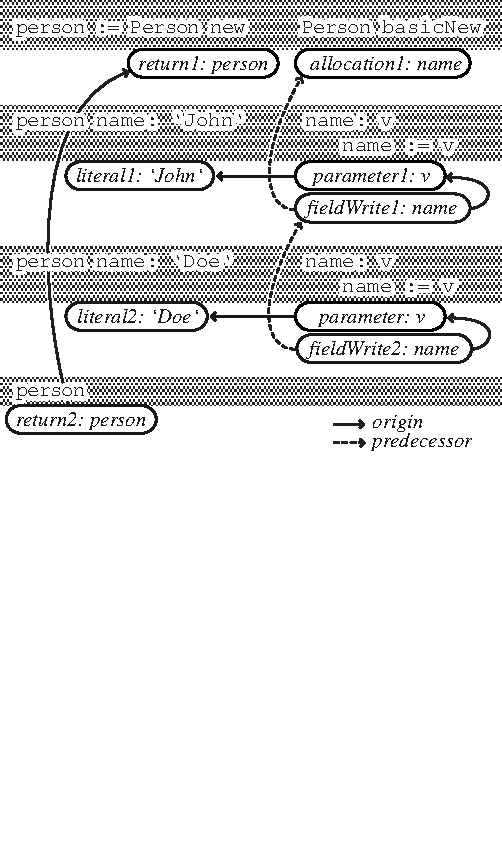
\includegraphics{objectflow.pdf}
	\caption{The objectflow interpreter.}
	\label{fig:objectflow}
\end{figure}

\begin{figure}[h]
	\centering
	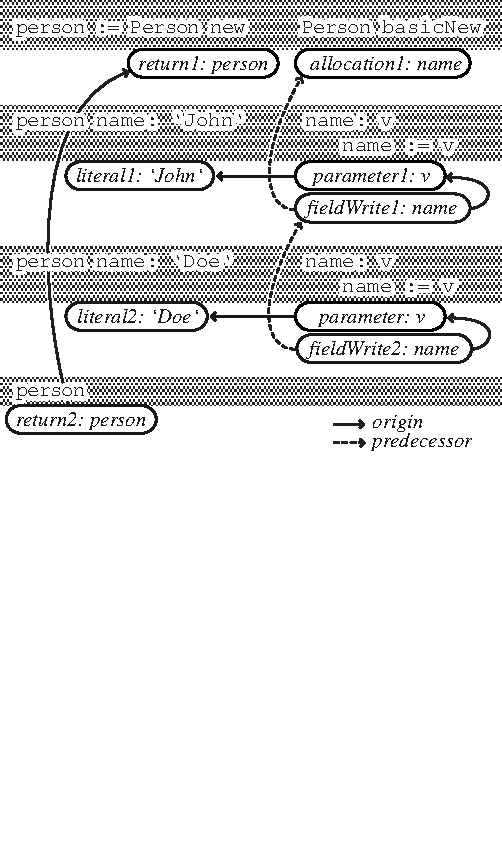
\includegraphics{objectflow.pdf}
	\caption{A Figure with only the h tag causing a warning}
	\label{fig:htWarning}
\end{figure}


\section{Ref-test}
\ref{sec:citetest} is the previous section and \ref{fig:htWarning} the
previous image.

% ===========================================================================

\bibliographystyle{abbrvnat}
\bibliography{test}

% ===========================================================================
\end{document}
